% Chapter 7: Seminar - Cointegration and VECM
% Quizzes, Practice Problems, and Discussion
% Bachelor program, Bucharest University of Economic Studies

\documentclass[9pt, aspectratio=169, t]{beamer}

% Ensure content fits on slides
\setbeamersize{text margin left=8mm, text margin right=8mm}

%=============================================================================
% THEME AND STYLE CONFIGURATION
%=============================================================================
\usetheme{default}
% Using default theme for clean header/footer control

% Color Palette (matching Redispatch PDF)
\definecolor{MainBlue}{RGB}{26, 58, 110}
\definecolor{AccentBlue}{RGB}{26, 58, 110}
\definecolor{IDAred}{RGB}{205, 0, 0}
\definecolor{DarkGray}{RGB}{51, 51, 51}
\definecolor{MediumGray}{RGB}{128, 128, 128}
\definecolor{LightGray}{RGB}{248, 248, 248}
\definecolor{VeryLightGray}{RGB}{235, 235, 235}
\definecolor{KeynoteGray}{RGB}{218, 218, 218}
\definecolor{SectionGray}{RGB}{120, 120, 120}
\definecolor{FooterGray}{RGB}{100, 100, 100}
\definecolor{Crimson}{RGB}{220, 53, 69}
\definecolor{Forest}{RGB}{46, 125, 50}
\definecolor{Amber}{RGB}{181, 133, 63}
\definecolor{Orange}{RGB}{230, 126, 34}
\definecolor{Purple}{RGB}{142, 68, 173}

% Gradient background (exact Keynote 315° gradient: white to RGB 218,218,218)
\setbeamertemplate{background}{%
    \begin{tikzpicture}[remember picture, overlay]
        \shade[shading=axis, shading angle=315,
        top color=white, bottom color=KeynoteGray]
        (current page.south west) rectangle (current page.north east);
    \end{tikzpicture}%
}
% Fallback solid color for compatibility
\setbeamercolor{background canvas}{bg=}

\setbeamercolor{palette primary}{bg=MainBlue, fg=white}
\setbeamercolor{palette secondary}{bg=MainBlue!85, fg=white}
\setbeamercolor{palette tertiary}{bg=MainBlue!70, fg=white}
\setbeamercolor{structure}{fg=MainBlue}
\setbeamercolor{title}{fg=IDAred}
\setbeamercolor{frametitle}{fg=IDAred, bg=}
\setbeamercolor{block title}{bg=MainBlue, fg=white}
\setbeamercolor{block body}{bg=VeryLightGray, fg=DarkGray}
\setbeamercolor{block title alerted}{bg=Crimson, fg=white}
\setbeamercolor{block body alerted}{bg=Crimson!8, fg=DarkGray}
\setbeamercolor{block title example}{bg=Forest, fg=white}
\setbeamercolor{block body example}{bg=Forest!8, fg=DarkGray}
\setbeamercolor{item}{fg=MainBlue}

% Footer colors (override Madrid theme blue)
\setbeamercolor{author in head/foot}{fg=FooterGray, bg=}
\setbeamercolor{title in head/foot}{fg=FooterGray, bg=}
\setbeamercolor{date in head/foot}{fg=FooterGray, bg=}
\setbeamercolor{section in head/foot}{fg=FooterGray, bg=}
\setbeamercolor{subsection in head/foot}{fg=FooterGray, bg=}

% Bullet styles (apply everywhere including blocks)
\setbeamertemplate{itemize item}{\color{MainBlue}$\boxdot$}
\setbeamertemplate{itemize subitem}{\color{MainBlue}$\blacktriangleright$}
\setbeamertemplate{itemize subsubitem}{\color{MainBlue}\tiny$\bullet$}
\setbeamertemplate{itemize/enumerate body begin}{\normalsize}
\setbeamertemplate{itemize/enumerate subbody begin}{\normalsize}

% Item spacing - compact style
\setlength{\leftmargini}{10pt}       % Level 1: minimal indent
\setlength{\leftmarginii}{10pt}      % Level 2: minimal additional indent
% Compact list spacing (zero extra space before/after lists in blocks)
\makeatletter
\def\@listi{\leftmargin\leftmargini \topsep 0pt \parsep 0pt \itemsep 0pt}
\def\@listii{\leftmargin\leftmarginii \topsep 0pt \parsep 0pt \itemsep 0pt}
\makeatother

\setbeamertemplate{navigation symbols}{}

%=============================================================================
% CUSTOM HEADLINE
%=============================================================================
\setbeamertemplate{headline}{%
    \vskip10pt%
    \hbox to \paperwidth{%
        \hskip0.5cm%
        {\small\color{FooterGray}\renewcommand{\hyperlink}[2]{##2}\insertsectionhead}%
        \hfill%
        \textcolor{FooterGray}{\small\insertframenumber}%
        \hskip0.5cm%
    }%
    \vskip4pt%
    {\color{FooterGray}\hrule height 0.4pt}%
}

%=============================================================================
% CUSTOM FOOTER
%=============================================================================
\usepackage{fontawesome5}

\setbeamertemplate{footline}{%
    {\color{FooterGray}\hrule height 0.4pt}%
    \vskip4pt%
    \hbox to \paperwidth{%
        \hskip0.5cm%
        \textcolor{FooterGray}{\small Time Series Analysis and Forecasting}%
        \hfill%
        \raisebox{-0.1em}{%
            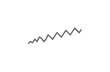
\begin{tikzpicture}[x=0.08em, y=0.08em, line width=0.4pt]
                \draw[FooterGray] (0,3) -- (1,4) -- (2,3.5) -- (3,5) -- (4,4) -- (5,6) -- (6,5.5) -- (7,4) -- (8,5) -- (9,7) -- (10,6) -- (11,5) -- (12,6.5) -- (13,8) -- (14,7) -- (15,6) -- (16,7.5) -- (17,9) -- (18,8) -- (19,7) -- (20,8.5) -- (21,10) -- (22,9) -- (23,8) -- (24,9.5);
            \end{tikzpicture}%
        }%
        \hskip0.5cm%
    }%
    \vskip6pt%
}

%=============================================================================
% PACKAGES
%=============================================================================
\usepackage[utf8]{inputenc}
\usepackage[T1]{fontenc}
\usepackage[english]{babel}
\usepackage{amsmath, amssymb, amsthm}
\usepackage{mathtools}
\usepackage{bm}
\usepackage{tikz}
\usetikzlibrary{arrows.meta, positioning, shapes, calc, decorations.pathreplacing, shadings}
\usepackage{booktabs}
\usepackage{multirow}
\usepackage{array}
\usepackage{graphicx}
\usepackage{hyperref}
\usepackage{colortbl}
\hypersetup{colorlinks=true, linkcolor=MainBlue, urlcolor=MainBlue}
\graphicspath{{../../logos/}{../../charts/}}
\hfuzz=2pt  % Suppress tiny overfull warnings (<2pt)
\vfuzz=2pt  % Suppress tiny vertical overfull warnings (<2pt)

%=============================================================================
% QUANTLET COMMAND
%=============================================================================
\newcommand{\quantlet}[2]{%
    \hfill\href{#2}{%
        \raisebox{-0.15em}{\includegraphics[height=0.7em]{ql_logo.png}}%
        \textcolor{MainBlue}{\tiny\ #1}%
    }%
}

%=============================================================================
% CENTRED MINIPAGE
%=============================================================================
\newenvironment{cminipage}[1]{%
    \par\noindent\hfill\begin{minipage}{#1}\ignorespaces
}{%
    \end{minipage}\hfill\null\par
}

%=============================================================================
% CUSTOM COMMANDS
%=============================================================================
\newcommand{\E}{\mathbb{E}}
\newcommand{\Var}{\text{Var}}
\newcommand{\Cov}{\text{Cov}}
\newcommand{\bY}{\mathbf{Y}}
\newcommand{\bA}{\mathbf{A}}
\newcommand{\bepsilon}{\boldsymbol{\varepsilon}}
\newcommand{\bvarepsilon}{\boldsymbol{\varepsilon}}
\newcommand{\bc}{\mathbf{c}}
\newcommand{\bPi}{\boldsymbol{\Pi}}
\newcommand{\balpha}{\boldsymbol{\alpha}}
\newcommand{\bbeta}{\boldsymbol{\beta}}
\newcommand{\bGamma}{\boldsymbol{\Gamma}}

%=============================================================================
% TITLE INFORMATION
%=============================================================================
\title[Chapter 7: Seminar]{Chapter 7: Seminar --- Cointegration \& VECM}
\subtitle{Bachelor program Faculty of Cybernetics, Statistics and Economic Informatics, Bucharest University of Economic Studies, Romania}
\author[Prof. dr. Daniel Traian Pele]{Prof. dr. Daniel Traian Pele\\[0.2cm]\footnotesize\texttt{danpele@ase.ro}}
\institute{Bucharest University of Economic Studies}
\date{Academic Year 2025--2026}

\begin{document}

%=============================================================================
% TITLE SLIDE
%=============================================================================
\begin{frame}[plain]
    \begin{tikzpicture}[remember picture, overlay]
        \fill[IDAred] (current page.north west) rectangle ([yshift=-0.15cm]current page.north east);
        \node[anchor=north west] at ([xshift=0.5cm, yshift=-0.3cm]current page.north west) {
            \href{https://www.ase.ro}{\includegraphics[height=1.1cm]{ase_logo.png}}
        };
        \node[anchor=north] at ([yshift=-0.3cm]current page.north) {
            \href{https://ai4efin.ase.ro}{\includegraphics[height=1.1cm]{ai4efin_logo.png}}
        };
        \node[anchor=north east] at ([xshift=-0.5cm, yshift=-0.3cm]current page.north east) {
            \href{https://www.digital-finance-msca.com}{\includegraphics[height=1.1cm]{msca_logo.png}}
        };
    \end{tikzpicture}
    \vfill
    \begin{center}
        {\Large\textcolor{MediumGray}{Time Series Analysis and Forecasting}}\\[0.3cm]
        {\Huge\textbf{\textcolor{MainBlue}{Chapter 7: Cointegration \& VECM}}}\\[0.5cm]
        {\Large\textcolor{IDAred}{Seminar}}
    \end{center}
    \vfill

    \begin{tikzpicture}[remember picture, overlay]
        \fill[IDAred] (current page.south west) rectangle ([yshift=0.15cm]current page.south east);
        \node[anchor=south west] at ([xshift=0.5cm, yshift=0.8cm]current page.south west) {
            \href{https://theida.net}{\includegraphics[height=0.9cm]{ida_logo.png}}
        };
        \node[anchor=south] at ([xshift=-3cm, yshift=0.8cm]current page.south) {
            \href{https://blockchain-research-center.com}{\includegraphics[height=0.9cm]{brc_logo.png}}
        };
        \node[anchor=south] at ([yshift=0.8cm]current page.south) {
            \href{https://quantinar.com}{\includegraphics[height=0.9cm]{qr_logo.png}}
        };
        \node[anchor=south] at ([xshift=3cm, yshift=0.8cm]current page.south) {
            \href{https://quantlet.com}{\includegraphics[height=0.9cm]{ql_logo.png}}
        };
        \node[anchor=south east] at ([xshift=-0.5cm, yshift=0.8cm]current page.south east) {
            \href{https://ipe.ro/new}{\includegraphics[height=0.9cm]{acad_logo.png}}
        };
    \end{tikzpicture}
\end{frame}

%=============================================================================
% OUTLINE
%=============================================================================
\begin{frame}{Seminar Outline}
    \begin{cminipage}{0.95\textwidth}
    \textbf{\large Seminar structure:}

    \vspace{0.4cm}

    \begin{enumerate}
        \item[\textcolor{MainBlue}{\textbf{1.}}] \textbf{Review Quiz} -- Knowledge check
        \vspace{0.15cm}
        \item[\textcolor{MainBlue}{\textbf{2.}}] \textbf{True/False Questions} -- Conceptual checks
        \vspace{0.15cm}
        \item[\textcolor{MainBlue}{\textbf{3.}}] \textbf{Practice Problems} -- Applied practice
        \vspace{0.15cm}
        \item[\textcolor{MainBlue}{\textbf{4.}}] \textbf{Worked Examples} -- Detailed solutions
        \vspace{0.15cm}
        \item[\textcolor{MainBlue}{\textbf{5.}}] \textbf{Discussion Topics} -- Critical thinking
        \vspace{0.15cm}
        \item[\textcolor{MainBlue}{\textbf{6.}}] \textbf{AI-Assisted Exercises} -- Applied artificial intelligence
    \end{enumerate}
    \end{cminipage}
\end{frame}

%=============================================================================
% SECTION 1: REVIEW QUIZ
%=============================================================================
\section{Review Quiz}

\begin{frame}{Quiz 1: Cointegration Definition}
    \begin{alertblock}{Question}
        Two I(1) variables $X_t$ and $Y_t$ are cointegrated if:
    \end{alertblock}

    \vspace{0.3cm}

    \begin{enumerate}[A)]
        \item They are both stationary
        \item Their sum is I(2)
        \item A linear combination of them is I(0)
        \item They have the same mean
    \end{enumerate}

    \vspace{0.5cm}
    \begin{flushright}\textit{Answer on next slide...}\end{flushright}
\end{frame}

\begin{frame}{Quiz 1: Answer}
    \begin{cminipage}{0.95\textwidth}
    \begin{exampleblock}{Answer: C -- A linear combination is I(0)}
        \begin{center}
            \includegraphics[width=0.85\textwidth, height=0.60\textheight, keepaspectratio]{ch6_quiz1_cointegration.pdf}
        \end{center}
        \vspace{-0.2cm}
        {\footnotesize
        \textbf{Key}: $Y_t - \beta X_t \sim I(0)$ means they share a common stochastic trend. The linear combination (spread) is stationary even though both series are non-stationary.
        }
    \end{exampleblock}
    \quantlet{TSA\_ch7\_cointegration}{https://github.com/QuantLet/TSA/tree/main/TSA_ch7/TSA_ch7_cointegration}
    \end{cminipage}
\end{frame}

\begin{frame}{Quiz 2: Spurious Regression}
    \begin{alertblock}{Question}
        When regressing one independent random walk on another, you typically get:
    \end{alertblock}

    \vspace{0.3cm}

    \begin{enumerate}[A)]
        \item Low $R^2$ and insignificant coefficients
        \item High $R^2$ and significant coefficients (spurious!)
        \item Zero coefficients
        \item Undefined results
    \end{enumerate}

    \vspace{0.5cm}
    \begin{flushright}\textit{Answer on next slide...}\end{flushright}
\end{frame}

\begin{frame}[shrink=5]{Quiz 2: Answer}
    \begin{cminipage}{0.95\textwidth}
    \begin{exampleblock}{Answer: B -- High $R^2$ and significant coefficients (spurious!)}
        \begin{center}
            \includegraphics[width=0.85\textwidth, height=0.60\textheight, keepaspectratio]{ch6_quiz2_spurious.pdf}
        \end{center}
        \vspace{-0.2cm}
        {\footnotesize
        \textbf{Granger-Newbold (1974)}: Regressing unrelated I(1) series gives misleading results. Rule of thumb: If $R^2 > DW$, suspect spurious regression!
        \faIcon{globe} Real-world examples: \href{https://www.tylervigen.com/spurious-correlations}{\texttt{tylervigen.com/spurious-correlations}}
        }
    \end{exampleblock}
    \quantlet{TSA\_ch7\_spurious}{https://github.com/QuantLet/TSA/tree/main/TSA_ch7/TSA_ch7_spurious}
    \end{cminipage}
\end{frame}

\begin{frame}{Quiz 3: Engle-Granger Test}
    \begin{alertblock}{Question}
        In the Engle-Granger two-step method, what do you test in step 2?
    \end{alertblock}

    \vspace{0.3cm}

    \begin{enumerate}[A)]
        \item Whether the original variables are stationary
        \item Whether the regression residuals have a unit root
        \item Whether the coefficients are significant
        \item Whether the $R^2$ is high enough
    \end{enumerate}

    \vspace{0.5cm}
    \begin{flushright}\textit{Answer on next slide...}\end{flushright}
\end{frame}

\begin{frame}{Quiz 3: Answer}
    \begin{cminipage}{0.95\textwidth}
    \begin{exampleblock}{Answer: B -- Whether residuals have unit root}
        \textbf{Step 1}: Run OLS: $Y_t = \alpha + \beta X_t + e_t$, save residuals $\hat{e}_t$

        \vspace{0.2cm}
        \textbf{Step 2}: ADF test on residuals: $\Delta \hat{e}_t = \rho \hat{e}_{t-1} + \ldots$
        \begin{itemize}
            \item $H_0$: $\rho = 0$ (unit root $\Rightarrow$ no cointegration)
            \item $H_1$: $\rho < 0$ (stationary $\Rightarrow$ cointegration!)
        \end{itemize}

        \vspace{0.2cm}
        \textbf{Important}: Use Engle-Granger critical values, not standard ADF!
    \end{exampleblock}
    \quantlet{TSA\_ch7\_engle\_granger}{https://github.com/QuantLet/TSA/tree/main/TSA_ch7/TSA_ch7_engle_granger}
    \end{cminipage}
\end{frame}

\begin{frame}{Quiz 4: Johansen Test Advantage}
    \begin{alertblock}{Question}
        The main advantage of Johansen over Engle-Granger is:
    \end{alertblock}

    \vspace{0.3cm}

    \begin{enumerate}[A)]
        \item It's simpler to compute
        \item It can detect multiple cointegrating relationships
        \item It doesn't require data
        \item It always finds cointegration
    \end{enumerate}

    \vspace{0.5cm}
    \begin{flushright}\textit{Answer on next slide...}\end{flushright}
\end{frame}

\begin{frame}{Quiz 4: Answer}
    \begin{cminipage}{0.95\textwidth}
    \begin{exampleblock}{Answer: B -- Can detect multiple cointegrating relationships}
        \begin{center}
            \includegraphics[width=0.85\textwidth, height=0.52\textheight, keepaspectratio]{ch6_quiz4_johansen.pdf}
        \end{center}
        \vspace{-0.3cm}
        {\footnotesize
        \textbf{Johansen advantages}: Tests for $r = 0, 1, \ldots, k-1$ cointegrating vectors; MLE (more efficient); no need to choose dependent variable.
        }
    \end{exampleblock}
    \quantlet{TSA\_ch7\_johansen}{https://github.com/QuantLet/TSA/tree/main/TSA_ch7/TSA_ch7_johansen}
    \end{cminipage}
\end{frame}

\begin{frame}{Quiz 5: Rank of $\bPi$}
    \begin{alertblock}{Question}
        In a VECM with $k=3$ variables, if $\text{rank}(\bPi) = 2$, this means:
    \end{alertblock}

    \vspace{0.3cm}

    \begin{enumerate}[A)]
        \item No cointegration
        \item One cointegrating relationship
        \item Two cointegrating relationships
        \item All variables are stationary
    \end{enumerate}

    \vspace{0.5cm}
    \begin{flushright}\textit{Answer on next slide...}\end{flushright}
\end{frame}

\begin{frame}{Quiz 5: Answer}
    \begin{cminipage}{0.95\textwidth}
    \begin{exampleblock}{Answer: C -- Two cointegrating relationships}
        \textbf{Rank interpretation} for $k$ variables:
        \begin{itemize}
            \item $\text{rank}(\bPi) = 0$: No cointegration (use VAR in differences)
            \item $0 < \text{rank}(\bPi) = r < k$: $r$ cointegrating vectors (use VECM)
            \item $\text{rank}(\bPi) = k$: All variables are I(0) (use VAR in levels)
        \end{itemize}

        \vspace{0.2cm}
        \textbf{With $k=3$ and $r=2$}:
        \begin{itemize}
            \item Two equilibrium relationships
            \item Only $k - r = 1$ common stochastic trend
        \end{itemize}
    \end{exampleblock}
    \quantlet{TSA\_ch7\_vecm}{https://github.com/QuantLet/TSA/tree/main/TSA_ch7/TSA_ch7_vecm}
    \end{cminipage}
\end{frame}

\begin{frame}{Quiz 6: VECM Structure}
    \begin{alertblock}{Question}
        In the VECM equation $\Delta \bY_t = \bc + \balpha\bbeta'\bY_{t-1} + \ldots$, what does $\balpha$ represent?
    \end{alertblock}

    \vspace{0.3cm}

    \begin{enumerate}[A)]
        \item The cointegrating vectors
        \item The adjustment (loading) coefficients
        \item The short-run dynamics
        \item The error variance
    \end{enumerate}

    \vspace{0.5cm}
    \begin{flushright}\textit{Answer on next slide...}\end{flushright}
\end{frame}

\begin{frame}[shrink=5]{Quiz 6: Answer}
    \begin{cminipage}{0.95\textwidth}
    \begin{exampleblock}{Answer: B -- The adjustment (loading) coefficients}
        \begin{center}
            \includegraphics[width=0.85\textwidth, height=0.50\textheight, keepaspectratio]{ch6_quiz6_adjustment.pdf}
        \end{center}
        \vspace{-0.2cm}
        {\footnotesize
        \textbf{$\bPi = \balpha\bbeta'$}:
        \begin{itemize}
            \item $\bbeta$ = cointegrating vectors (define equilibrium)
            \item $\balpha$ = adjustment speeds (how fast each variable corrects)
        \end{itemize}
        }
    \end{exampleblock}
    \quantlet{TSA\_ch7\_ecm}{https://github.com/QuantLet/TSA/tree/main/TSA_ch7/TSA_ch7_ecm}
    \end{cminipage}
\end{frame}

\begin{frame}{Quiz 7: Error Correction Term}
    \begin{alertblock}{Question}
        If $Y_t - \beta X_t$ is the cointegrating relation and this term is positive, what happens?
    \end{alertblock}

    \vspace{0.3cm}

    \begin{enumerate}[A)]
        \item $Y$ is above equilibrium; $Y$ should decrease (if $\alpha < 0$)
        \item $Y$ is below equilibrium; $Y$ should increase
        \item Nothing, error correction doesn't affect levels
        \item Both variables increase
    \end{enumerate}

    \vspace{0.5cm}
    \begin{flushright}\textit{Answer on next slide...}\end{flushright}
\end{frame}

\begin{frame}{Quiz 7: Answer}
    \begin{cminipage}{0.95\textwidth}
    \begin{exampleblock}{Answer: A -- $Y$ above equilibrium; decreases if $\alpha < 0$}
        \textbf{Error correction mechanism}:
        $$\Delta Y_t = \alpha(Y_{t-1} - \beta X_{t-1}) + \ldots$$

        \begin{itemize}
            \item If $Y_{t-1} - \beta X_{t-1} > 0$: $Y$ is ``too high''
            \item With $\alpha < 0$: $\Delta Y_t < 0$ (Y decreases toward equilibrium)
            \item This is the ``error correction'' pulling $Y$ back
        \end{itemize}

        \vspace{0.2cm}
        \textbf{Sign convention}: $\alpha$ should be negative for the dependent variable to move back toward equilibrium.
    \end{exampleblock}
    \quantlet{TSA\_ch7\_error\_correction}{https://github.com/QuantLet/TSA/tree/main/TSA_ch7/TSA_ch7_error_correction}
    \end{cminipage}
\end{frame}

\begin{frame}{Quiz 8: Weak Exogeneity}
    \begin{alertblock}{Question}
        If $\alpha_2 = 0$ in a bivariate VECM, this means:
    \end{alertblock}

    \vspace{0.3cm}

    \begin{enumerate}[A)]
        \item There is no cointegration
        \item Variable 2 does not adjust to disequilibrium (weakly exogenous)
        \item Variable 1 does not adjust
        \item Both variables are stationary
    \end{enumerate}

    \vspace{0.5cm}
    \begin{flushright}\textit{Answer on next slide...}\end{flushright}
\end{frame}

\begin{frame}{Quiz 8: Answer}
    \begin{exampleblock}{Answer: B -- Variable 2 is weakly exogenous}
        \textbf{Weak exogeneity}: Variable doesn't respond to disequilibrium.

        \vspace{0.2cm}
        \textbf{Example: Interest rates}
        \begin{itemize}
            \item Long rate ($R_t$) often weakly exogenous ($\alpha_R \approx 0$)
            \item Short rate ($r_t$) adjusts to spread ($\alpha_r < 0$)
            \item Interpretation: Central bank adjusts short rate to maintain term structure
        \end{itemize}

        \vspace{0.2cm}
        \textbf{Implication}: Can estimate single equation for the adjusting variable.
    \end{exampleblock}
\end{frame}

\begin{frame}{Quiz 9: Trace Test}
    \begin{alertblock}{Question}
        The Johansen trace test with $H_0: r \leq 1$ vs $H_1: r > 1$ tests whether:
    \end{alertblock}

    \vspace{0.3cm}

    \begin{enumerate}[A)]
        \item There is exactly one cointegrating vector
        \item There are at most one cointegrating vectors
        \item There are more than one cointegrating vectors
        \item All eigenvalues are zero
    \end{enumerate}

    \vspace{0.5cm}
    \begin{flushright}\textit{Answer on next slide...}\end{flushright}
\end{frame}

\begin{frame}{Quiz 9: Answer}
    \begin{exampleblock}{Answer: B/C -- $H_0$: at most 1; $H_1$: more than 1}
        \textbf{Sequential testing procedure}:
        \begin{enumerate}
            \item Test $H_0: r = 0$ vs $H_1: r > 0$
            \item If rejected, test $H_0: r \leq 1$ vs $H_1: r > 1$
            \item Continue until fail to reject...
        \end{enumerate}

        \vspace{0.2cm}
        \textbf{Trace statistic}:
        $$\lambda_{\text{trace}}(r) = -T \sum_{i=r+1}^{k} \ln(1 - \hat{\lambda}_i)$$

        Reject $H_0$ if trace statistic $>$ critical value.
    \end{exampleblock}
\end{frame}

\begin{frame}{Quiz 10: VECM vs VAR in Differences}
    \begin{alertblock}{Question}
        If variables are cointegrated, using VAR in first differences instead of VECM:
    \end{alertblock}

    \vspace{0.3cm}

    \begin{enumerate}[A)]
        \item Gives identical results
        \item Is more efficient
        \item Loses long-run information (misspecified)
        \item Is the preferred approach
    \end{enumerate}

    \vspace{0.5cm}
    \begin{flushright}\textit{Answer on next slide...}\end{flushright}
\end{frame}

\begin{frame}{Quiz 10: Answer}
    \begin{exampleblock}{Answer: C -- Loses long-run information}
        \textbf{Granger Representation Theorem}: If cointegrated, VECM representation exists and should be used.

        \vspace{0.2cm}
        \begin{center}
        \begin{tabular}{lcc}
            \toprule
            & \textbf{VAR($\Delta$)} & \textbf{VECM} \\
            \midrule
            Long-run equilibrium & Lost & Preserved \\
            Error correction & No & Yes \\
            Forecasts (long-run) & Poor & Better \\
            \bottomrule
        \end{tabular}
        \end{center}

        \vspace{0.2cm}
        \textbf{Bottom line}: Differencing removes the long-run relationship that cointegration represents!
    \end{exampleblock}
\end{frame}

%=============================================================================
% TRUE/FALSE QUESTIONS
%=============================================================================
\section{True/False Questions}

\begin{frame}{True/False Questions}
    Determine if each statement is True or False:

    \vspace{0.3cm}
    \begin{enumerate}
        \item Cointegration requires all variables to be I(1).
        \item The cointegrating vector is unique.
        \item Spurious regression has low Durbin-Watson statistic.
        \item In VECM, both $\alpha$ coefficients must be non-zero.
        \item Johansen test requires choosing a dependent variable.
        \item The number of common trends = $k - r$.
    \end{enumerate}

    \vspace{0.3cm}
    \begin{flushright}\textit{Answers on next slide...}\end{flushright}
\end{frame}

\begin{frame}{True/False: Solutions}
    {\small
    \begin{enumerate}\setlength{\itemsep}{1pt}
        \item Cointegration requires all variables to be I(1). \hfill \textcolor{Forest}{\textbf{TRUE}}

        {\footnotesize \textcolor{MediumGray}{Standard CI(1,1) case: all variables I(1), linear combination I(0).}}

        \item The cointegrating vector is unique. \hfill \textcolor{Crimson}{\textbf{FALSE}}

        {\footnotesize \textcolor{MediumGray}{Unique only up to scalar multiplication. Usually normalized ($\beta_1 = 1$).}}

        \item Spurious regression has low Durbin-Watson statistic. \hfill \textcolor{Forest}{\textbf{TRUE}}

        {\footnotesize \textcolor{MediumGray}{$DW \approx 0$ indicates highly autocorrelated residuals (non-stationary).}}

        \item In VECM, both $\alpha$ coefficients must be non-zero. \hfill \textcolor{Crimson}{\textbf{FALSE}}

        {\footnotesize \textcolor{MediumGray}{One can be zero (weak exogeneity). At least one must be non-zero.}}

        \item Johansen test requires choosing a dependent variable. \hfill \textcolor{Crimson}{\textbf{FALSE}}

        {\footnotesize \textcolor{MediumGray}{That's Engle-Granger. Johansen treats all variables symmetrically.}}

        \item The number of common trends = $k - r$. \hfill \textcolor{Forest}{\textbf{TRUE}}

        {\footnotesize \textcolor{MediumGray}{$k$ variables, $r$ cointegrating relations $\Rightarrow$ $k-r$ common stochastic trends.}}
    \end{enumerate}
    }
\end{frame}

%=============================================================================
% SECTION 2: PRACTICE PROBLEMS
%=============================================================================
\section{Practice Problems}

\begin{frame}{Problem 1: Cointegration Identification}
    \begin{block}{Exercise}
        You have quarterly data on consumption ($C_t$) and income ($Y_t$). ADF tests show both are I(1). The regression $C_t = 0.85 Y_t + e_t$ gives residuals with ADF statistic $= -3.92$. The 5\% Engle-Granger critical value for 2 variables is $-3.34$.

        \vspace{0.2cm}
        Are $C_t$ and $Y_t$ cointegrated?
    \end{block}

    \vspace{0.5cm}
    \begin{flushright}\textit{Answer on next slide...}\end{flushright}
\end{frame}

\begin{frame}{Problem 1: Solution}
    \begin{cminipage}{0.95\textwidth}
    \begin{exampleblock}{Solution: Yes, they are cointegrated}
        \textbf{Test}: $H_0$: No cointegration (residuals have unit root)

        \vspace{0.2cm}
        \textbf{ADF statistic}: $-3.92$

        \textbf{Critical value (5\%)}: $-3.34$

        \vspace{0.2cm}
        Since $-3.92 < -3.34$, we \textbf{reject} $H_0$ at 5\% level.

        \vspace{0.2cm}
        \textbf{Conclusion}: Residuals are stationary $\Rightarrow$ Cointegration exists!

        \vspace{0.2cm}
        \textbf{Interpretation}: Consumption and income share a common trend. The cointegrating vector is approximately $(1, -0.85)$, consistent with permanent income hypothesis.
    \end{exampleblock}
    \quantlet{TSA\_ch7\_engle\_granger\_test}{https://github.com/QuantLet/TSA/tree/main/TSA_ch7/TSA_ch7_engle_granger_test}
    \end{cminipage}
\end{frame}

\begin{frame}{Problem 2: VECM Interpretation}
    \begin{block}{Exercise}
        A VECM for short rate ($r_t$) and long rate ($R_t$) gives:
        \begin{align*}
            \Delta r_t &= 0.01 - 0.25(r_{t-1} - R_{t-1}) + \ldots \\
            \Delta R_t &= 0.005 - 0.02(r_{t-1} - R_{t-1}) + \ldots
        \end{align*}
        Interpret the adjustment coefficients.
    \end{block}

    \vspace{0.5cm}
    \begin{flushright}\textit{Answer on next slide...}\end{flushright}
\end{frame}

\begin{frame}{Problem 2: Solution}
    \begin{cminipage}{0.95\textwidth}
    \begin{exampleblock}{Solution}
        \textbf{Error correction term}: $(r_{t-1} - R_{t-1})$ = spread

        \vspace{0.2cm}
        \textbf{Short rate} ($\alpha_r = -0.25$):
        \begin{itemize}
            \item When spread is positive (short $>$ long), short rate decreases
            \item 25\% of disequilibrium corrected per period
            \item Short rate actively adjusts
        \end{itemize}

        \vspace{0.2cm}
        \textbf{Long rate} ($\alpha_R = -0.02$):
        \begin{itemize}
            \item Very small adjustment coefficient
            \item Long rate is nearly weakly exogenous
            \item Mostly driven by expectations, not error correction
        \end{itemize}

        \vspace{0.2cm}
        \textbf{Economic interpretation}: Central bank (short rate) adjusts to maintain yield curve.
    \end{exampleblock}
    \quantlet{TSA\_ch7\_vecm\_interpretation}{https://github.com/QuantLet/TSA/tree/main/TSA_ch7/TSA_ch7_vecm_interpretation}
    \end{cminipage}
\end{frame}

\begin{frame}{Problem 3: Johansen Test Results}
    \begin{block}{Exercise}
        Johansen trace test for 3 variables gives:
        \begin{center}
        \begin{tabular}{lcc}
            \toprule
            $H_0$ & Trace Stat & 5\% CV \\
            \midrule
            $r = 0$ & 45.2 & 29.8 \\
            $r \leq 1$ & 18.1 & 15.5 \\
            $r \leq 2$ & 3.2 & 3.8 \\
            \bottomrule
        \end{tabular}
        \end{center}
        What is the cointegrating rank?
    \end{block}

    \vspace{0.5cm}
    \begin{flushright}\textit{Answer on next slide...}\end{flushright}
\end{frame}

\begin{frame}{Problem 3: Solution}
    \begin{cminipage}{0.95\textwidth}
    \begin{exampleblock}{Solution: Rank = 2}
        \textbf{Sequential testing}:
        \begin{enumerate}
            \item $H_0: r = 0$: $45.2 > 29.8$ $\Rightarrow$ \textbf{Reject} (at least 1)
            \item $H_0: r \leq 1$: $18.1 > 15.5$ $\Rightarrow$ \textbf{Reject} (at least 2)
            \item $H_0: r \leq 2$: $3.2 < 3.8$ $\Rightarrow$ \textbf{Fail to reject}
        \end{enumerate}

        \vspace{0.2cm}
        \textbf{Conclusion}: $r = 2$ cointegrating relationships

        \vspace{0.2cm}
        \textbf{Implications}:
        \begin{itemize}
            \item Two equilibrium relationships among 3 variables
            \item Only $3 - 2 = 1$ common stochastic trend
            \item Use VECM with 2 error correction terms
        \end{itemize}
    \end{exampleblock}
    \quantlet{TSA\_ch7\_johansen\_test}{https://github.com/QuantLet/TSA/tree/main/TSA_ch7/TSA_ch7_johansen_test}
    \end{cminipage}
\end{frame}

%=============================================================================
% SECTION 3: WORKED EXAMPLES
%=============================================================================
\section{Worked Examples}

\begin{frame}{Example: Term Structure of Interest Rates}
    {\small
    \begin{block}{Economic Theory}
        Expectations hypothesis: $R_t^{(n)} = \frac{1}{n}\sum_{i=0}^{n-1} E_t[r_{t+i}] + \text{premium}$

        If premium is constant $\Rightarrow$ spread $(R_t - r_t)$ should be stationary.
    \end{block}
    \begin{exampleblock}{Typical Findings}
        \begin{itemize}\setlength{\itemsep}{0pt}
            \item Both rates are I(1) (confirmed by ADF)
            \item Johansen test: $r = 1$ cointegrating vector
            \item Cointegrating vector $\approx (1, -1)$: spread is stationary
            \item Short rate adjusts ($\alpha_r < 0$), long rate weakly exogenous
        \end{itemize}
    \end{exampleblock}
    \begin{block}{Policy Implication}
        Central bank controls short rate; long rate driven by expectations.
    \end{block}
    }
\end{frame}

\begin{frame}{Example: Purchasing Power Parity}
    {\small
    \begin{block}{PPP Theory}
        $e_t = p_t - p_t^*$ (log exchange rate = price differential)

        Real exchange rate: $q_t = e_t - p_t + p_t^*$ should be stationary (long-run PPP)
    \end{block}
    \begin{exampleblock}{Empirical Challenges}
        \begin{itemize}\setlength{\itemsep}{0pt}
            \item Unit root tests: $e_t$, $p_t$, $p_t^*$ all I(1)
            \item Cointegration tests: Mixed results depending on sample
            \item Half-life of PPP deviations: 3-5 years (slow adjustment)
            \item Weak exogeneity: Exchange rate often doesn't adjust
        \end{itemize}
    \end{exampleblock}
    \begin{alertblock}{PPP Puzzle}
        Real exchange rate is highly persistent---slow mean reversion is hard to explain with standard models.
    \end{alertblock}
    }
\end{frame}

\begin{frame}{Example: Pairs Trading Strategy}
    \vspace{-0.3cm}
    {\small
    \begin{block}{Idea}
        Find cointegrated stocks $\Rightarrow$ trade the stationary spread
    \end{block}
    \begin{exampleblock}{Implementation Steps}
        \begin{enumerate}\setlength{\itemsep}{0pt}
            \item \textbf{Identify pairs}: Test cointegration (e.g., Coca-Cola \& Pepsi)
            \item \textbf{Estimate spread}: $z_t = P_A - \beta P_B$
            \item \textbf{Trading rules}:
            \begin{itemize}
                \item $z_t > \mu + 2\sigma$: Sell A, Buy B (spread too wide)
                \item $z_t < \mu - 2\sigma$: Buy A, Sell B (spread too narrow)
                \item Exit when $z_t \approx \mu$
            \end{itemize}
        \end{enumerate}
    \end{exampleblock}
    \begin{alertblock}{Risks}
        Cointegration can break down; spread may not revert; transaction costs.
    \end{alertblock}
    }
\end{frame}

\begin{frame}{Python Cointegration Analysis: Key Functions}
    {\footnotesize
    \begin{block}{Essential Libraries}
        \texttt{from statsmodels.tsa.stattools import coint, adfuller} \\
        \texttt{from statsmodels.tsa.vector\_ar.vecm import coint\_johansen, VECM}
    \end{block}

    \begin{block}{Workflow}
        \begin{enumerate}\setlength{\itemsep}{0pt}
            \item Unit root tests: \texttt{adfuller(series)}
            \item Engle-Granger: \texttt{coint(y, x)} returns test stat \& p-value
            \item Johansen: \texttt{coint\_johansen(data, det\_order, k\_ar\_diff)}
            \item Fit VECM: \texttt{model = VECM(data, k\_ar\_diff=2, coint\_rank=1)}
            \item Results: \texttt{results = model.fit()}
        \end{enumerate}
    \end{block}

    \begin{alertblock}{Note}
        Complete working examples are provided in the Jupyter notebooks.
    \end{alertblock}
    }
\end{frame}

%=============================================================================
% SECTION 4: DISCUSSION TOPICS
%=============================================================================
\section{Discussion Topics}

\begin{frame}{Discussion: Cointegration vs Correlation}
    {\small
    \begin{alertblock}{Key Question}
        Two series are highly correlated. Are they cointegrated?
    \end{alertblock}
    \begin{block}{Answer: Not necessarily!}
        \begin{itemize}\setlength{\itemsep}{0pt}
            \item \textbf{Correlation}: Measures co-movement (can be spurious for I(1))
            \item \textbf{Cointegration}: Requires stationary linear combination
        \end{itemize}
    \end{block}
    \begin{exampleblock}{Example}
        Two independent random walks can have correlation $> 0.9$ purely by chance (spurious correlation). But they're NOT cointegrated---their spread is also I(1).

        \vspace{0.2cm}
        \textbf{Cointegration} implies a meaningful long-run equilibrium relationship.
    \end{exampleblock}
    }
\end{frame}

\begin{frame}{Discussion: Choosing Deterministic Components}
    {\small
    \begin{alertblock}{Key Question}
        Johansen test has 5 cases for deterministics. Which to choose?
    \end{alertblock}
    \begin{block}{Guidelines}
        \begin{enumerate}\setlength{\itemsep}{0pt}
            \item \textbf{No constant, no trend}: Rarely used (requires mean-zero data)
            \item \textbf{Constant in CE only}: Level series, no drift
            \item \textbf{Constant unrestricted}: Most common for economic data
            \item \textbf{Trend in CE}: Series have deterministic trends
            \item \textbf{Trend unrestricted}: Trending differences (uncommon)
        \end{enumerate}
    \end{block}
    \begin{exampleblock}{Practical Advice}
        Start with Case 3 (constant unrestricted). Check sensitivity to specification. Use economic reasoning: do levels have trends?
    \end{exampleblock}
    }
\end{frame}

%=============================================================================
% SECTION 5: EXERCISES
%=============================================================================
\section{AI-Assisted Exercises}

\begin{frame}{Take-Home Exercises}
    {\footnotesize
    \begin{enumerate}\setlength{\itemsep}{2pt}
        \item \textbf{Theoretical}: Show that if $Y_t$ and $X_t$ are both random walks with the same innovation, they are cointegrated.

        \item \textbf{Computation}: Given VECM estimates:
            \begin{align*}
                \Delta Y_t &= 0.5 - 0.3(Y_{t-1} - 2X_{t-1}) + 0.2\Delta Y_{t-1} \\
                \Delta X_t &= 0.1 + 0.1(Y_{t-1} - 2X_{t-1}) + 0.4\Delta X_{t-1}
            \end{align*}
            \begin{itemize}\setlength{\itemsep}{0pt}
                \item What is the cointegrating vector?
                \item Which variable adjusts more quickly?
                \item What is the long-run equilibrium relationship?
            \end{itemize}

        \item \textbf{Applied}: Download 10-year and 3-month Treasury rates:
            \begin{itemize}\setlength{\itemsep}{0pt}
                \item Test for unit roots; Test for cointegration (Engle-Granger and Johansen)
                \item Estimate VECM; Interpret adjustment coefficients
            \end{itemize}

        \item \textbf{Critical Thinking}: Why might PPP hold in the long run but not short run?
    \end{enumerate}
    }
\end{frame}

\begin{frame}{Exercise Solutions Hints}
    {\footnotesize
    \begin{block}{Hints}
        \begin{enumerate}\setlength{\itemsep}{1pt}
            \item If $Y_t = Y_{t-1} + \varepsilon_t$ and $X_t = X_{t-1} + \varepsilon_t$ (same shock), then $Y_t - X_t = Y_0 - X_0$ is constant (stationary).

            \item From the VECM:
                \begin{itemize}\setlength{\itemsep}{0pt}
                    \item Cointegrating vector: $(1, -2)$ (normalized on $Y$)
                    \item $Y$ adjusts faster: $|\alpha_Y| = 0.3 > |\alpha_X| = 0.1$
                    \item Long-run: $Y = 2X$ (when EC term = 0)
                \end{itemize}

            \item For interest rates:
                \begin{itemize}\setlength{\itemsep}{0pt}
                    \item Both typically I(1); spread usually stationary
                    \item Expect one cointegrating vector with $(1, -1)$
                    \item Short rate typically adjusts; long rate often weakly exogenous
                \end{itemize}

            \item PPP deviations: Transportation costs, non-traded goods, sticky prices, tariffs, market segmentation all slow adjustment but don't prevent long-run convergence.
        \end{enumerate}
    \end{block}
    }
\end{frame}

%=============================================================================
% SUMMARY
%=============================================================================
\begin{frame}{Key Takeaways from This Seminar}
    \vspace{-0.5cm}
    {\footnotesize
    \begin{block}{Main Points}
        \begin{enumerate}\setlength{\itemsep}{0pt}
            \item \textbf{Cointegration}: I(1) variables with stationary linear combination
            \item \textbf{Spurious regression}: High $R^2$ without cointegration is meaningless
            \item \textbf{Engle-Granger}: Simple, but only one cointegrating vector
            \item \textbf{Johansen}: Multiple vectors, MLE, more powerful
        \end{enumerate}
    \end{block}
    \begin{block}{VECM Insights}
        \begin{itemize}\setlength{\itemsep}{0pt}
            \item $\bbeta$ defines equilibrium; $\balpha$ determines adjustment speed
            \item Weak exogeneity ($\alpha = 0$): Variable doesn't respond to disequilibrium
            \item Always use VECM (not VAR in differences) when cointegrated
        \end{itemize}
    \end{block}
    \begin{alertblock}{Remember}
        Cointegration is about \textbf{long-run equilibrium}, not just correlation!
    \end{alertblock}
    }
\end{frame}


\begin{frame}{AI Exercise: Critical Thinking}
    \begin{cminipage}{0.95\textwidth}
    \vspace{-0.3cm}
    \begin{block}{\footnotesize Prompt to test in ChatGPT / Claude / Copilot}
        {\footnotesize
        ``Download oil spot and futures prices (CL=F, BZ=F). Test for cointegration and estimate a VECM model. Can I use the spread for a pairs trading strategy?''
        }
    \end{block}
    \vspace{-2mm}
    {\footnotesize
    \textbf{Exercise}:
    \begin{enumerate}\setlength{\itemsep}{0pt}
        \item Run the prompt in an LLM of your choice and critically analyze the response.
        \item Does the AI test the order of integration of each series before testing for cointegration?
        \item Johansen or Engle-Granger test? Does the AI justify the choice?
        \item Is the cointegrating rank ($r$) correctly interpreted?
        \item Does the pairs trading strategy account for transaction costs and model risk?
    \end{enumerate}
    }
    \vspace{-2mm}
    \begin{alertblock}{}
        {\footnotesize \textbf{Warning}: AI-generated code may run without errors and look professional. \textit{That does not mean it is correct.}}
    \end{alertblock}
    \end{cminipage}
\end{frame}

%=============================================================================
% THANK YOU
%=============================================================================
\begin{frame}{}
    \begin{cminipage}{0.95\textwidth}
    \centering
    \Huge\textcolor{IDAred}{Thank You!}

    \vspace{1cm}

    \Large\textcolor{MainBlue}{Questions?}

    \vspace{0.8cm}

    \normalsize
    Seminar materials are available at: \url{https://danpele.github.io/Time-Series-Analysis/}

    \vspace{0.2cm}

    \href{https://quantlet.com}{\raisebox{-0.15em}{\includegraphics[height=0.8em]{ql_logo.png}} Quantlet} \hspace{0.5cm}
    \href{https://quantinar.com}{\raisebox{-0.15em}{\includegraphics[height=0.8em]{qr_logo.png}} Quantinar}
    \end{cminipage}
\end{frame}

%=============================================================================
% BIBLIOGRAPHY
%=============================================================================
\begin{frame}{Bibliography I}
    \begin{block}{Fundamental Textbooks}
        {\small
        \begin{itemize}
            \item Hyndman, R.J., \& Athanasopoulos, G. (2021). \textit{Forecasting: Principles and Practice}, 3rd ed., OTexts.
            \item Shumway, R.H., \& Stoffer, D.S. (2017). \textit{Time Series Analysis and Its Applications}, 4th ed., Springer.
            \item Brockwell, P.J., \& Davis, R.A. (2016). \textit{Introduction to Time Series and Forecasting}, 3rd ed., Springer.
        \end{itemize}
        }
    \end{block}

    \begin{exampleblock}{Financial Time Series}
        {\small
        \begin{itemize}
            \item Tsay, R.S. (2010). \textit{Analysis of Financial Time Series}, 3rd ed., Wiley.
            \item Franke, J., H\"ardle, W.K., \& Hafner, C.M. (2019). \textit{Statistics of Financial Markets}, 4th ed., Springer.
        \end{itemize}
        }
    \end{exampleblock}
\end{frame}

\begin{frame}{Bibliography II}
    \begin{block}{Modern Approaches and Machine Learning}
        {\small
        \begin{itemize}
            \item Nielsen, A. (2019). \textit{Practical Time Series Analysis}, O'Reilly Media.
            \item Petropoulos, F., et al. (2022). \textit{Forecasting: Theory and Practice}, International Journal of Forecasting.
            \item Makridakis, S., Spiliotis, E., \& Assimakopoulos, V. (2020). The M4 Competition, International Journal of Forecasting.
        \end{itemize}
        }
    \end{block}

    \begin{exampleblock}{Online Resources and Code}
        {\small
        \begin{itemize}
            \item \textbf{Quantlet}: \url{https://quantlet.com} --- Code repository for statistics
            \item \textbf{Quantinar}: \url{https://quantinar.com} --- Platform for learning quantitative methods
            \item \textbf{GitHub TSA}: \url{https://github.com/QuantLet/TSA} --- Python code for this seminar
        \end{itemize}
        }
    \end{exampleblock}
\end{frame}

\end{document}
